% 图 35.2 —— 由 `checks/emit_hand.py` 自动拼出（probe 精测 + prims2 图元分解）
%%
% ⚠ 这是**稿子不是成品**：跑 `checks/checkhand.py 35.2` 看指标 + 看叠合图。
%%
%% ⚠ 待核：
%   · 本图 probe 报出阴影族 1 个 —— **本脚本不生成阴影**（要照原书手写）；prims2 的 strokes 里可能含阴影线，核对时留意别画重
%   · 可疑字形 1 项（空心圈 ⊙ 常被认成字母 o）—— 见文件末
%%
\documentclass[12pt]{standalone}
\usepackage{fontspec}
\setsansfont{Arial}
\newfontfamily\mfallback{DejaVu Sans}
\usepackage{tikz}
\begin{document}
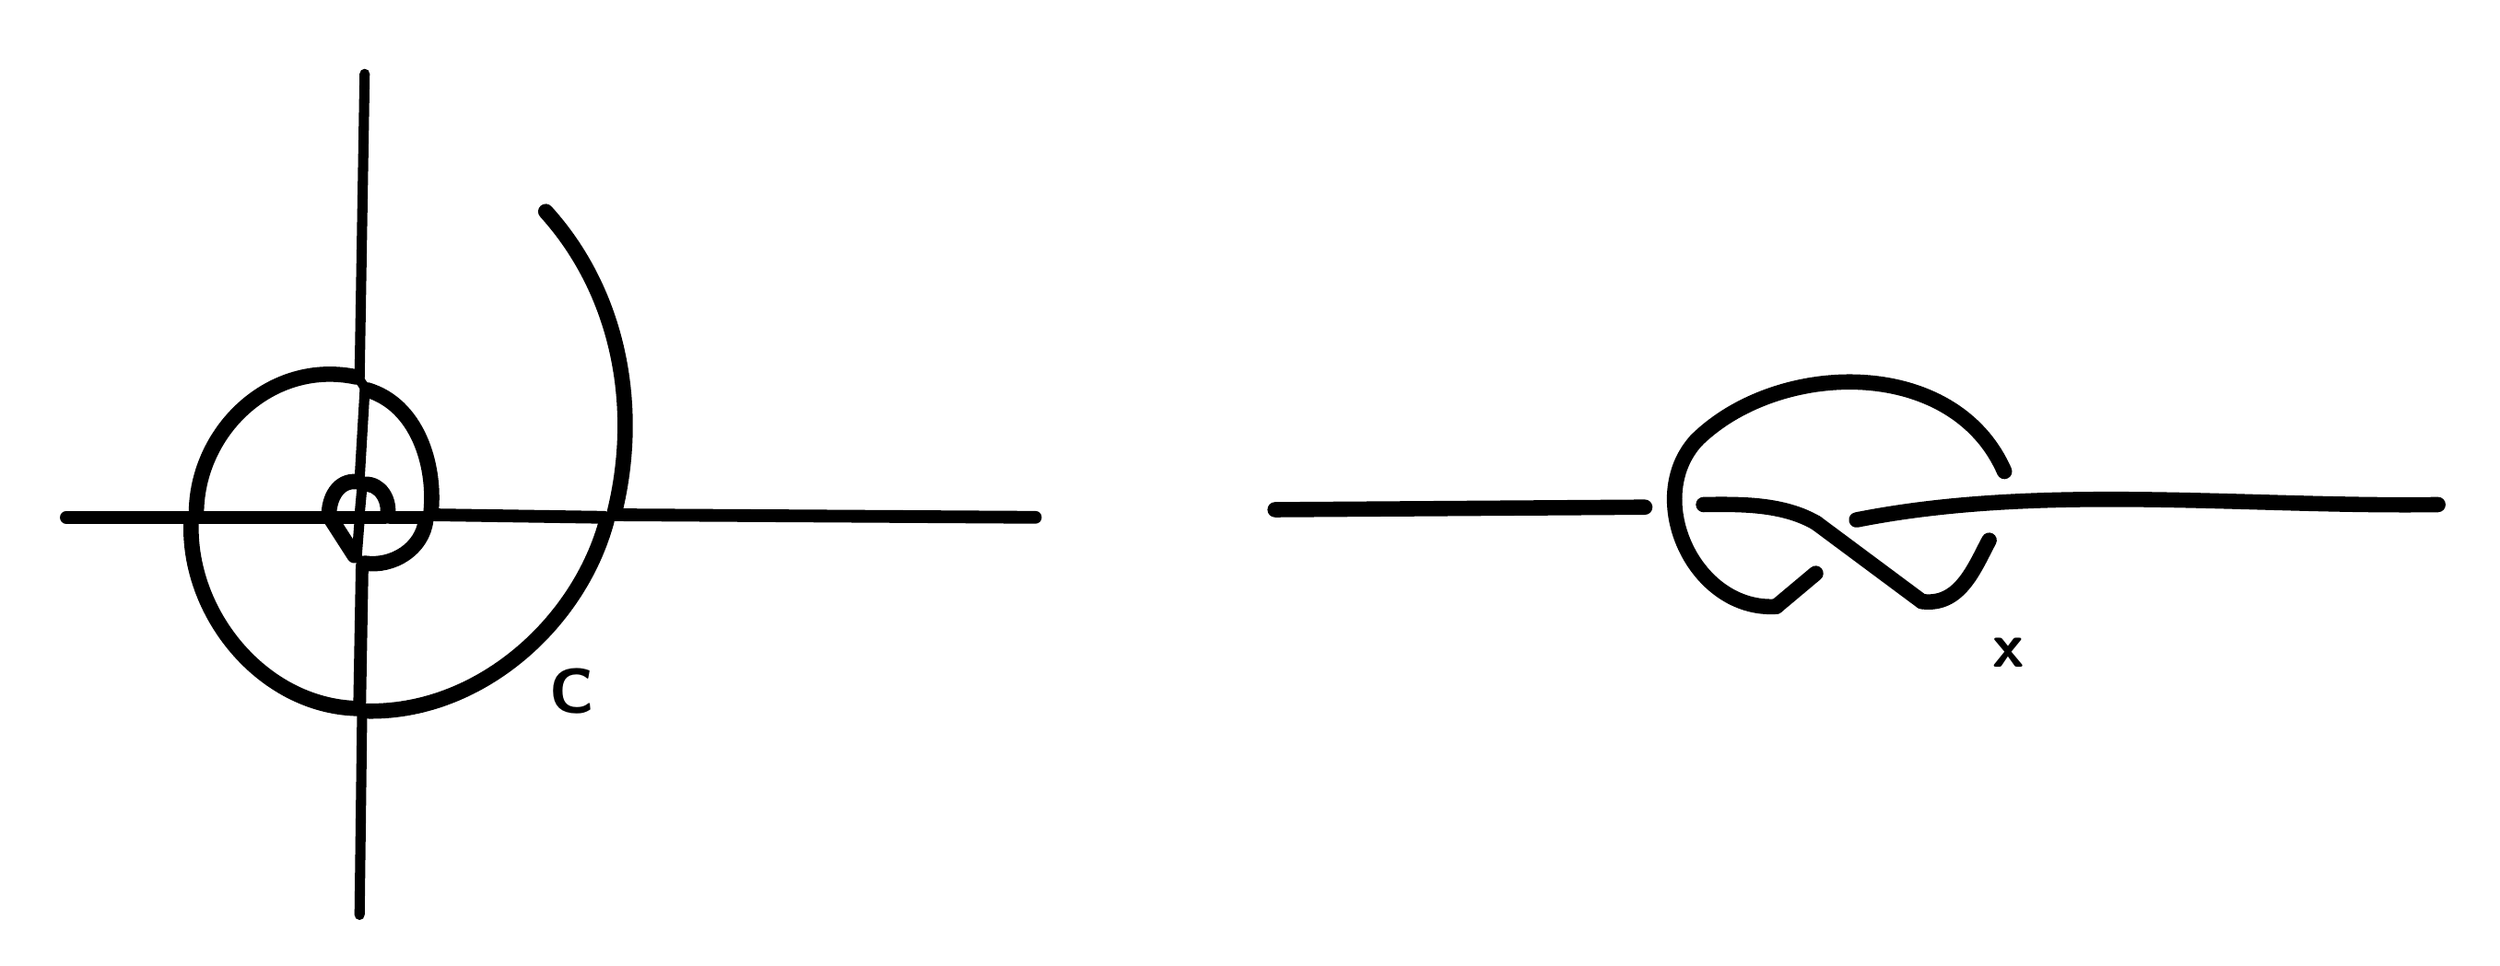
\begin{tikzpicture}[x=1pt, y=-1pt, line width=5.0pt, line cap=round, line join=round]

  %% ════ 直线段（prims2 的 strokes）════
  \draw[line width=5.0pt] (118.0,193.0) -- (68.0,193.0);
  \draw[line width=6.0pt] (743.6,226.0) -- (702.2,195.2);
  \draw[line width=4.0pt] (131.0,192.0) -- (132.0,181.0);
  \draw[line width=5.0pt] (141.0,193.0) -- (132.0,193.0);
  \draw[line width=4.0pt] (132.0,270.0) -- (131.0,349.0);
  \draw[line width=5.0pt] (143.0,193.0) -- (156.0,193.0);
  \draw[line width=5.0pt] (132.0,212.0) -- (131.0,268.0);
  \draw[line width=5.0pt] (227.0,193.0) -- (159.0,192.0);
  \draw[line width=4.0pt] (133.0,144.0) -- (131.0,178.0);
  \draw[line width=5.0pt] (231.0,192.0) -- (396.0,193.0);
  \draw[line width=4.0pt] (130.0,207.0) -- (131.0,194.0);
  \draw[line width=6.0pt] (129.0,208.0) -- (120.0,194.0);
  \draw[line width=5.0pt] (16.0,193.0) -- (64.0,193.0);
  \draw[line width=4.0pt] (131.0,138.0) -- (133.0,19.0);
  \draw[line width=5.0pt] (121.0,193.0) -- (130.0,193.0);
  \draw[line width=3.8pt] (131.0,139.0) -- (133.0,142.0);
  \draw[line width=6.0pt] (635.0,189.0) -- (490.0,190.0);
  \draw[line width=6.0pt] (686.5,228.0) -- (702.0,215.0);

  %% ════ 曲线（prims2 的 curves —— 三段式，坐标同为 (y,x)）════
  \draw[line width=6.0pt] (718.0,194.0) .. controls (790.5,179.6) and (870.6,189.1) .. (946.0,188.0);
  \draw[line width=6.0pt] (133.0,211.0) .. controls (144.2,212.6) and (155.7,205.3) .. (157.0,194.0);
  \draw[line width=6.0pt] (130.0,268.0) .. controls (92.7,267.0) and (63.1,230.2) .. (65.0,194.0);
  \draw[line width=6.0pt] (770.0,202.0) .. controls (764.3,212.6) and (758.6,228.1) .. (743.6,226.0);
  \draw[line width=6.0pt] (702.2,195.2) .. controls (689.1,187.6) and (672.6,187.8) .. (658.0,188.0);
  \draw[line width=6.0pt] (67.0,192.0) .. controls (66.7,159.7) and (95.9,130.6) .. (130.0,138.0);
  \draw[line width=6.0pt] (204.0,73.0) .. controls (232.7,104.7) and (241.2,149.5) .. (231.0,191.0);
  \draw[line width=6.0pt] (159.0,191.0) .. controls (160.9,172.0) and (153.4,148.7) .. (134.0,143.0);
  \draw[line width=6.0pt] (133.0,269.0) .. controls (177.3,270.4) and (217.1,235.0) .. (228.0,194.0);
  \draw[line width=6.0pt] (119.0,192.0) .. controls (119.0,185.6) and (122.5,178.3) .. (130.0,179.0);
  \draw[line width=6.0pt] (142.0,192.0) .. controls (142.9,186.2) and (139.2,179.7) .. (133.0,180.0);
  \draw[line width=6.0pt] (776.0,175.0) .. controls (756.1,129.5) and (687.3,131.3) .. (655.3,162.7);
  \draw[line width=6.0pt] (655.3,162.7) .. controls (634.1,185.8) and (654.6,230.0) .. (686.5,228.0);

  %% ════ 标签（probe 直接给的 \node 行）════
  %% ⚠ 全部补了 fill=white：文字在最上层，否则与曲线交叉干扰
     \node[anchor=center,inner sep=0pt,fill=white,font=\fontsize{38.9}{48.7}\selectfont] at (777.8,246.1) {\textsf{\textbf{\textit{x}}}};   % box(766,232,21,23)
     \node[anchor=center,inner sep=0pt,fill=white,font=\fontsize{32.9}{41.2}\selectfont] at (214.3,261.3) {\textsf{\textbf{\textit{C}}}};   % box(203,249,21,24)

  % 钉死画布：否则超出的图元/控制点会把页面撑大，1:1 回比就失准
  \pgfresetboundingbox
  \path[use as bounding box] (0,0) rectangle (960,359);
\end{tikzpicture}
\end{document}

% ⚠ 待核清单（probe 拿不准，人眼过一遍）：
%   · 未识别/跳过：⑤ 跳过/未识别的字形
